%%%%%%%%%%%%%%%%%%%%%%%%%%%%%%%%%%%%%%%%%
% Stylish Article
% LaTeX Template
% Version 2.1 (1/10/15)
%
% This template has been downloaded from:
% http://www.LaTeXTemplates.com
%
% Original author:
% Mathias Legrand (legrand.mathias@gmail.com) 
% With extensive modifications by:
% Vel (vel@latextemplates.com)
%
% License:
% CC BY-NC-SA 3.0 (http://creativecommons.org/licenses/by-nc-sa/3.0/)
%
%%%%%%%%%%%%%%%%%%%%%%%%%%%%%%%%%%%%%%%%%

%----------------------------------------------------------------------------------------
%	PACKAGES AND OTHER DOCUMENT CONFIGURATIONS
%----------------------------------------------------------------------------------------

\documentclass[fleqn,10pt]{SelfArx} % Document font size and equations flushed left

\usepackage[english]{babel} % Specify a different language here - english by default

\usepackage{lipsum} % Required to insert dummy text. To be removed otherwise

%----------------------------------------------------------------------------------------
%	COLUMNS
%----------------------------------------------------------------------------------------

\setlength{\columnsep}{0.55cm} % Distance between the two columns of text
\setlength{\fboxrule}{0.75pt} % Width of the border around the abstract

%----------------------------------------------------------------------------------------
%	COLORS
%----------------------------------------------------------------------------------------

\definecolor{color1}{RGB}{0,0,90} % Color of the article title and sections
\definecolor{color2}{RGB}{0,20,20} % Color of the boxes behind the abstract and headings

%----------------------------------------------------------------------------------------
%	HYPERLINKS
%----------------------------------------------------------------------------------------

\usepackage{hyperref} % Required for hyperlinks
\hypersetup{hidelinks,colorlinks,breaklinks=true,urlcolor=color2,citecolor=color1,linkcolor=color1,bookmarksopen=false,pdftitle={Title},pdfauthor={Author}}


\usepackage[demo]{graphicx}
\usepackage{caption}
\usepackage{subcaption}


%----------------------------------------------------------------------------------------
%	ARTICLE INFORMATION
%----------------------------------------------------------------------------------------

%\JournalInfo{Journal, Vol. XXI, No. 1, 1-5, 2013} % Journal information
%\Archive{Additional note} % Additional notes (e.g. copyright, DOI, review/research article)

\PaperTitle{Commssioning of an automated assembly system for the PS modules of the CMS phase II upgrade outer tracker.} % Article title

\Authors{James Keaveney\textsuperscript{1}*} % Authors
\affiliation{\textsuperscript{1}\textit{DESY, Hamburg Germany}} % Author affiliation
\affiliation{*\textbf{} james.keaveney@desy.de} % Corresponding author

\Keywords{} % Keywords - if you don't want any simply remove all the text between the curly brackets
\newcommand{\keywordname}{Keywords} % Defines the keywords heading name

%----------------------------------------------------------------------------------------
%	ABSTRACT
%----------------------------------------------------------------------------------------

\Abstract{
 The CMS phase II upgrade outer tracker is built from two types of modules (\emph{PS} and \emph{2S}) each consisting of two silicon sensors and associated electronics and mechanics. In the case of the PS module, the sensors be assembled to a precision of approximately 40 \mu$m.  In order to satisfy this requirement and a short module assembly time, an \emph{automated} assembly system is proposed. The student will join an ongoing effort to commission such a system based on a high-precision motion-stage integrated with pattern-recognition and mechanical control systems.  The student will work towards the demonstration of high precision assembly with short assembly times. 
 If time permits, the student will also commission a proposed module metrology system based on the same hardware.

 %extend the system to measure the alignment precision of assembled modules by realising a novel metrology concept that has been established already at the concept level. The student will develop mathematical and a software skills in addition to gaining experience with a state of the art lab environment. The final goal will be to confirm that the  automated assembly procedure achieves the alignment precision demanded by the module design.
}

%----------------------------------------------------------------------------------------

\begin{document}

\flushbottom % Makes all text pages the same height

\maketitle % Print the title and abstract box

\tableofcontents % Print the contents section

\thispagestyle{empty} % Removes page numbering from the first page

%----------------------------------------------------------------------------------------
%	ARTICLE CONTENTS
%----------------------------------------------------------------------------------------

\section*{Introduction} % The \section*{} command stops section numbering


\addcontentsline{toc}{section}{Introduction} % Adds this section to the table of contents
The CMS Phase-II Tracker will utilize two types of modules, 2S modules and PS modules. To achieve efficient rejection of low-pT particles throughout the Tracker volume, modules in different regions will make use of a few different sensor spacings. For 2S (PS) modules, spacings of 1.8 and 4 mm (1.6, 2.6 and 4 mm) are foreseen. These modules will be used in the end-cap disks as well as the central barrel region of the Tracker. An exploded view of a PS module is shown in Figure \ref{fig:PS}. In the PS module, the sensors are glued to a carbon-fibre reinforced Aluminium (AL-CF) spacers which act as spacers and provide the thermal conductance crucial for the cooling of the module. The structure consisting of the two sensors glued to two AL-CF spacers is henceforth referred to as the sensor sub-assembly (SSA). This project will focus on the assembly of the SSA only. The precision requirements of the SSA are shown in figure \ref{fig:precision}. For the PS module, the sensors must align to within 40 $\mu$m measured at the sensor's short edge. This corresponds to a rotational alignment tolerance of 0.8 mrad. 

\begin{figure*}[ht]\centering % Using \begin{figure*} makes the figure take up the entire width of the page
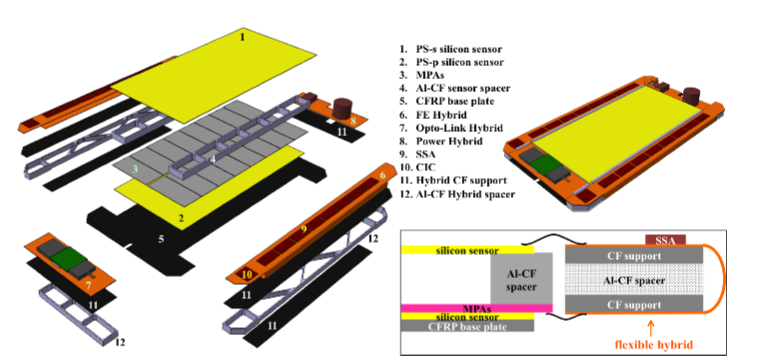
\includegraphics[width=\linewidth]{PS.png}
\caption{An exploded view of the PS module is shown.}
\label{fig:PS}
\end{figure*}

%------------------------------------------------

\section{Hardware}
The proposed automated assembly system consists of three sub-systems: the motion subsystem, the vision subsystem and the vacuum subsystem. 
The motion system provides the precise mechanical movements needed to arrange the components comprising the SSA. Movement of the components is achieved via mounting on the two moveable parts of the motion
system: the x-y-z and rotation stages. An custom-built AL tool known as the \emph{arm} is mounted on the x-y-z stage allowing mounting of components and thus movement of components in Cartesian coordinates. Components placed on the rotation stage may rotate in the horizontal plane with an angle $\phi$. The motion stages are controlled by a motion controller unit. All motion hardware is manufactured by Lang \footnote{Lang models: GT9-NSMA, LT-LBMA, RT5-NSMA} with motion precisions of 4 $\mu$m and $2$ mrad respectively. 

The vacuum system enables the mounting of components to the arm and rotation stage. It consists of a single pump providing vacuum to four switchable valves which in turn distribute vacuum to independent vacuum lines. The valves are switched to on(off) states by applying a control signal of 12 (0)V. The 12V signals are provided by a relay card. One vacuum line connects to the a \emph{pickup tool} which is mounted on the arm. The pickup tool consists of an ESD plastic block housing an inner vacuum chamber which distributed the vacuum to an array of downward facing suction cups which slightly protrude below the bottom side of the tool. A diagram of the pickup tool is shown in figure \ref{fig:pickuptool}. The \emph{pickup} procedure is performed by contacting the suction cups with the sensor, switching on the vacuum within the pickup tool and moving the arm directly upwards with the sensor attached. The \emph{setdown} procedure is performed by contacting the mounted sensor with the lower surface on which the component will be placed, switching off the vacuum in the pickup tool and moving the arm away. In order to avoid any movement of the component as the arm moves away, the component will be fixed in its setdown position with a separate array of upward-facing suction cups and independent vacuum line.

The vision system acquires images of components allow determination of their positions and orientations which is crucial for precise assembly. The vision system consists of two high-resolution cameras \footnote{IDS models}. One camera is mounted on the arm and is referred to as the \emph{mobile camera}. The other is mounted on a fixed vertical bracket in the assembly area and is known as the \emph{stationary camera}. Both cameras are fixed in a downward-facing orientation. The mobile camera acquires images immediately before pickups and immediately after setdowns in order to determine the positions of unmounted components. Conversely, the stationary camera acquires images of the sensors after pickups and before setdowns in order to determine their mounted orientation.


\begin{figure}[ht]\centering % Using \begin{figure*} makes the figure take up the entire width of the page
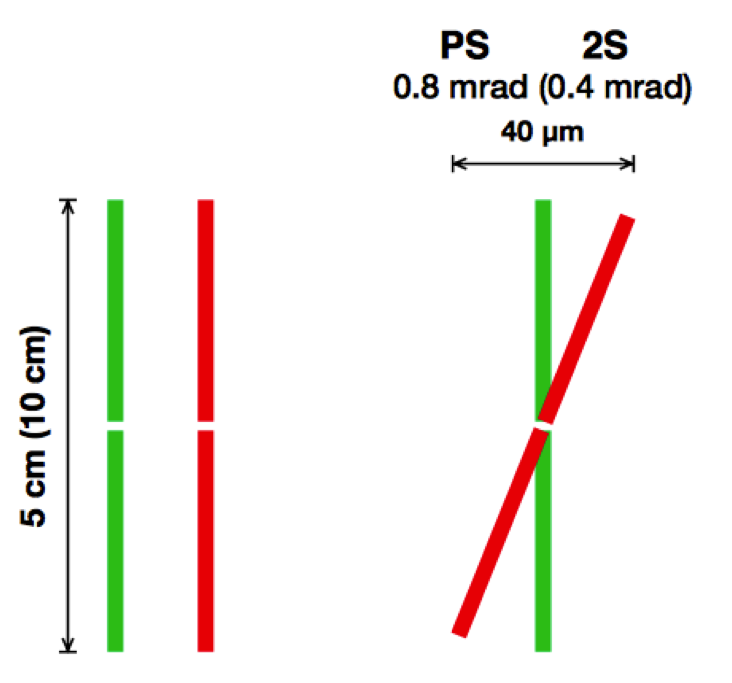
\includegraphics[width=0.5\linewidth]{Precision.png}
\caption{The precision requirements of the assembly of PS and 2S modules are shown.}
\label{fig:precision}
\end{figure}


\begin{figure}[ht]\centering % Using \begin{figure*} makes the figure take up the entire width of the page
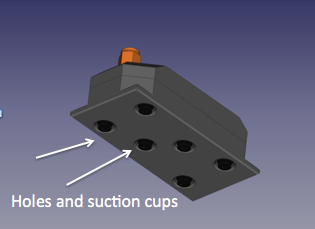
\includegraphics[width=\linewidth]{pickuptool.png}
\caption{DES}
\label{fig:pickuptool}
\end{figure}


\begin{figure}[ht]\centering % Using \begin{figure*} makes the figure take up the entire width of the page
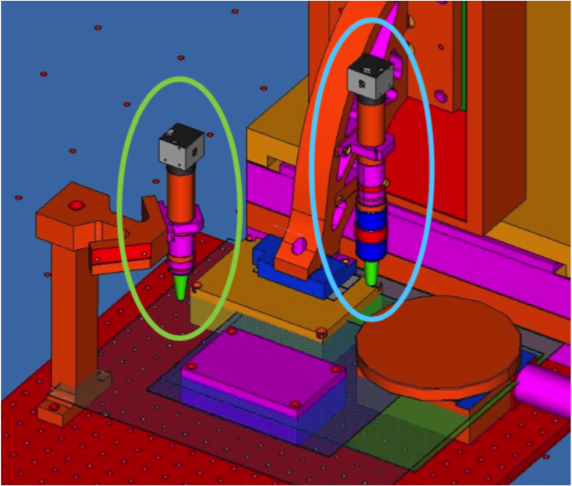
\includegraphics[width=\linewidth]{CADSetup.png}
\caption{A schematic of the assembly area is shown. The mobile(stationary) camera is circled in blue(green).}
\label{fig:cadsetup}
\end{figure}


\section{Software}
The control of the motion, vision and vacuum subsystems is integrated in a single software application henceforth referred to as \emph{PSAuto} \footnote{https://github.com/DESY-FH-ELab/cmstkmodlab.git}. PSAuto is entirely written in C++ and utilises the Qt framework version 4.8.7.  A schematic illustrating the integration of the subsystems with PSAuto is shown in figure \ref{fig:PSAuto}.


\begin{figure}[ht]\centering % Using \begin{figure*} makes the figure take up the entire width of the page
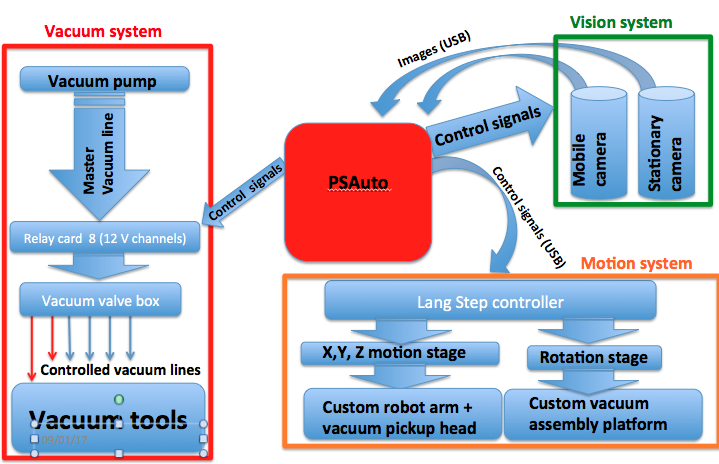
\includegraphics[width=\linewidth]{PSAuto.png}
\caption{A schematic of the integration of the motion, vision and vacuum subsystems via the PSAuto application is shown.}
\label{fig:PSAuto}
\end{figure}

\subsection{Pattern recognition}
An important task performed by PSAuto is the determination the location and \emph{planar orientation} \footnote{planar orientation is defined as the rotational orientation of the sensor in the horizontal (X-Z) plane} of the sensors during the assembly process. This is generally achieved in two basic steps: the independent determination of \emph{localised} positions and orientations of the four markers at the corners of the sensor and a global fit to these positions from which the final position and orientation of the entire sensor is extracted. 

This is done by processing the images of fiducial markers at the corners of the sensors acquired by the vision system with a Pattern Recognition algorithm. The markers are precisely positioned with respect to the strips or pixels or the sensors. Hence precise alignment of the markers ensures precise alignment of the pixels or strips.The algorithm takes raw images as input as returns the position and orientation of fiducial markers located at the corners of the PS sensors. T The pattern recognition algorithm utilises the \emph{OpenCV} package. The steps comprising the pattern recognition are now outined:

\textbf{1. Pre-processing of raw image}\\
The raw images from the camera are first converted from colour to black and white which is known as grayscaling in OpenCV. The pixels comprising the grayscaled image contain intensity information only in the form of a single number ranging from 0 to 255 describing the darkness of a shade of gray as opposed to the intensity and colour information contained in the pixels of a colour image. As the corner markers are based on simple shapes and not colours, the colour information is not helpful and is thus disregarded. The grayscaled image is then converted to a \emph{binary} image in which each pixel is either black or white in a process known as \emph{thresholding}. Thresholding simply converts each pixel of the image into a white(black) pixel if the intensity of the pixel is above(below) a pre-defined threshold. Thresholding serves to reduce the differences between images of identical sensors due to random \emph{noise} arising from dust and random differences in the surfaces of the patterned sensors. Examples of grayscaled and thresholded images of the same corner marker of a dummy PS sensor is shown in figures \ref{fig:grayscaledmarker} and \ref{fig:thresholdedmarker}. The optimal threshold will depend on the ambient lighting conditions around the assembly area and and the contrast of the fiducial markings on the sensors. Currently, values of 60 (90) are used for the master(template) image.

% \ref{fig:rawmarker}


%\begin{figure*}[ht]
%\centering
%\subfigure{\includegraphics[scale=0.38]{rawmarker.png}}
%\subfigure{\includegraphics[scale=0.38]{rawmarker.png}}
%\end{figure*}


\begin{figure}[!tbp]
  \centering
  \begin{minipage}[b]{0.23\textwidth}
    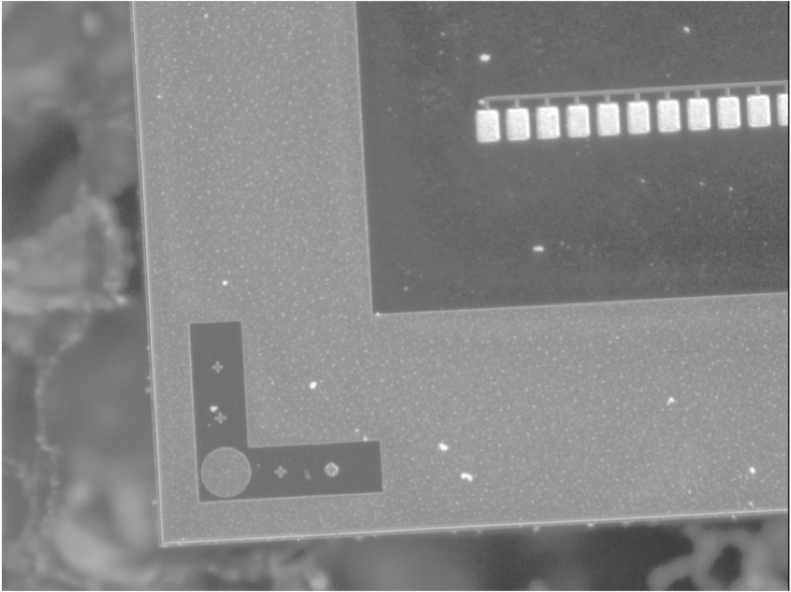
\includegraphics[width=\textwidth]{grayscaledmarker.png}
    \caption{Grayscaled}
    \label{fig:grayscaledmarker}
  \end{minipage}
%  \hfill
  \begin{minipage}[b]{0.23\textwidth}
    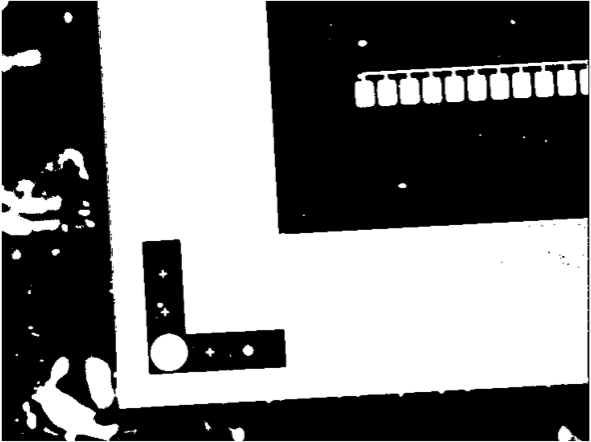
\includegraphics[width=\textwidth]{thresholdedmarker.png}
    \caption{Thresholded}
        \label{fig:thresholdedmarker}
  \end{minipage}
\end{figure}


\textbf{2. Determination of positions and planar orientations of fiducial markers.}\\
The position and orientation of the fiducial marker within the thresholded image is determined using a standard image processing technique known as \emph{template matching}. In template matching, parts of an master image that closely resemble a template image are located. In this case, the master image corresponds to the thresholded image of the fiducial marker and the template image corresponds to a thresholded image of a fiducial marker. 
Template matching proceeds by iteratively superimposing the template image at each point of the master image and calculating a metric which describes the similarity of the template image and the portion of the master image with which it coincides. The OpenCV package provides multiple options for the metric. Similar results are observed for each possible metric with the chosen metric based on the normalised squared difference between the intensities of coincident pixels of the master image and superimposed template \footnote{This metric is referred to as CV\_TM\_SQDIFF\_NORMED in OpenCV}. The point in the master image where the metric reaches a minimum represents the most probable location of the fiducial marker. In figure \ref{fig:templatematching} the determination of marker position with template matching is illustrated. In figure \ref{fig:templatematchingresult} the results of a test of the template matching algorithm using images of the a dummy sensor are shown. The most probable location of the marker as determined by the algorithm is indicated by the white rectangle. The observed location matches closely with expectation.

In order to deduce the orientation of the marker in the plane transverse to the optical axis of the camera, the matching procedure is repeated iteratively with different rotational transformations applied to the master image. In figure  For each iteration, the minimal value of the metric is recorded with the minimal metric value across all iterations denoted as $\alpha$. The planar orientation of the sensor is estimated as $-\alpha$. In figure \ref{fig:rotationextraction} a schematic illustrating the determination of the orientation is shown. In figure \ref{fig:rotationextractiongraph} a graph of the resultant minimised metric values versus the size of the angular transformation applied to the master image is shown. The graph corresponds to a test extraction performed with images of a dummy sensor where the sensor in the master image had a planar orientation of \approx$ 3.8 degrees. A clear minimum is observed at \approx$ 3.8 demonstrating the method' validity. Although the rather shallow minimum observed corresponds to a large uncertainty on the true orientation of $\mathcal{O}(0.5)$ degrees, it is expected that a more precise determination of the sensor orientation can be achieved when factors such as ambient light conditions, image focus and marker design are further optimised.

\begin{figure}[!tbp]
  \centering
  \begin{minipage}[b]{0.23\textwidth}
    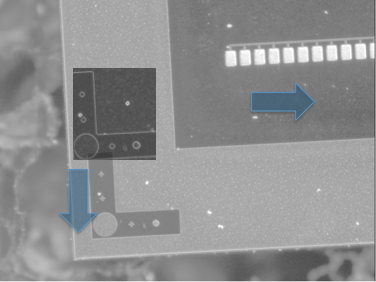
\includegraphics[width=\textwidth]{templatematching.png}
    \caption{The technique of template matching is illustrated. The blue arrows indicate the iterative calculation of a metric at each point of the master image.}
    \label{fig:templatematching}
  \end{minipage}
%  \hfill
  \begin{minipage}[b]{0.23\textwidth}
    \includegraphics[width=\textwidth]{patrec_tm_result.png}
    \caption{The result of a template matching routine on using test images is shown. The most probable location of the marker in the master image is outlined by the white rectangle.}
        \label{fig:templatematchingresult}
  \end{minipage}
\end{figure}

\begin{figure}[!tbp]
  \centering
  \begin{minipage}[b]{0.23\textwidth}
    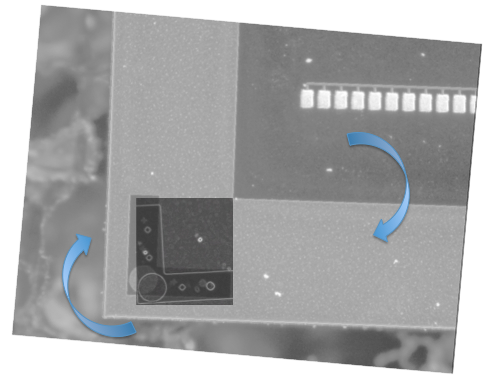
\includegraphics[width=\textwidth]{rotationextraction.png}
    \caption{A schematic illustrating the estimation of the sensors planar orientation is shown. The blue arrows indicate the iterative rotational transformations applied to the master image.}
    \label{fig:rotationextraction}
  \end{minipage}
%  \hfill
  \begin{minipage}[b]{0.23\textwidth}
    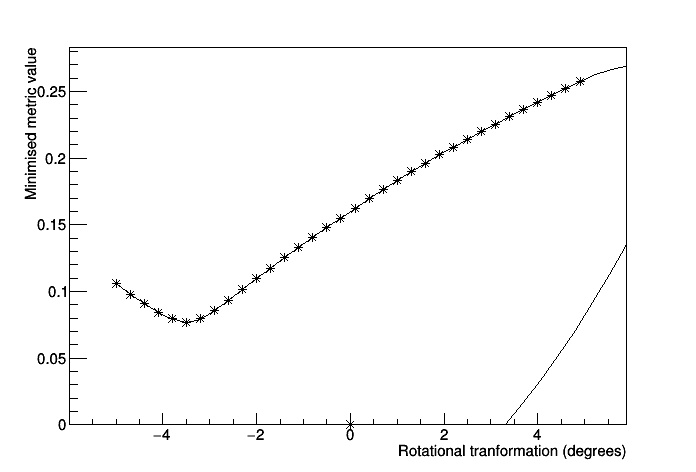
\includegraphics[width=\textwidth]{rotationextractiongraph.png}
    \caption{A graph of the minimised metric value versus the angular transformation applied to the master image is shown. A clear minimum at \approx$ 3.8 degrees is observed.}
        \label{fig:rotationextractiongraph}
  \end{minipage}
\end{figure}


\textbf{3. Location of other corners and extraction of final position and orientation.}\\
The procedure described in step 2 is repeated at each sensor corner. The planar orientations determined at given corner are used set the direction of movement needed for the motion
stage to automatically travel to an adjacent corner. The final position and orientation of the sensor is determined by a $\chi^{2}$ fit to the four (x,z) points. The orientation determined from the 
fit is cross-checked with the estimations of the orientation at the corners. If there is agreement between the fit and four corner orientations, the fit results are used.

\section{The assembly procedure}

List the X steps to assemble an SSA.




\lipsum[4] % Dummy text

\begin{equation}
\cos^3 \theta =\frac{1}{4}\cos\theta+\frac{3}{4}\cos 3\theta
\label{eq:refname2}
\end{equation}

\lipsum[5] % Dummy text

\begin{enumerate}[noitemsep] % [noitemsep] removes whitespace between the items for a compact look
\item First item in a list
\item Second item in a list
\item Third item in a list
\end{enumerate}

\subsection{Subsection}

\lipsum[6] % Dummy text

\paragraph{Paragraph} \lipsum[7] % Dummy text
\paragraph{Paragraph} \lipsum[8] % Dummy text

\subsection{Subsection}

\lipsum[9] % Dummy text


%------------------------------------------------

\section{Open tasks}

\subsection{Design and production of the assembly platform}
The assembly platform which will be attached the the rotation stage and provide a stable, flat surface on which the components will lie before, during and immediately after an attachment to other components. The platform must also distribute vacuum to allow fixing of the components to the lower surface during a setdown. The current design is shown in figure \ref{fig:assemblyplatform}





Two independent vacuum arrays are envisaged to allow fixing of both sensors and spacers.

\subsection{}

\subsection{Alignment Metrology}

\lipsum[10] % Dummy text

\subsection{Subsection}

\lipsum[11] % Dummy text

\begin{table}[hbt]
\caption{Table of Grades}
\centering
\begin{tabular}{llr}
\toprule
\multicolumn{2}{c}{Name} \\
\cmidrule(r){1-2}
First name & Last Name & Grade \\
\midrule
John & Doe & $7.5$ \\
Richard & Miles & $2$ \\
\bottomrule
\end{tabular}
\label{tab:label}
\end{table}

\subsubsection{Subsubsection}

\lipsum[12] % Dummy text

\begin{description}
\item[Word] Definition
\item[Concept] Explanation
\item[Idea] Text
\end{description}

\subsubsection{Subsubsection}

\lipsum[13] % Dummy text

\begin{itemize}[noitemsep] % [noitemsep] removes whitespace between the items for a compact look
\item First item in a list
\item Second item in a list
\item Third item in a list
\end{itemize}

\subsubsection{Subsubsection}

\lipsum[14] % Dummy text

\subsection{Subsection}

\lipsum[15-23] % Dummy text

%------------------------------------------------
\phantomsection
\section*{Acknowledgments} % The \section*{} command stops section numbering

\addcontentsline{toc}{section}{Acknowledgments} % Adds this section to the table of contents

So long and thanks for all the fish \cite{Figueredo:2009dg}.

%----------------------------------------------------------------------------------------
%	REFERENCE LIST
%----------------------------------------------------------------------------------------
\phantomsection
\bibliographystyle{unsrt}
\bibliography{sample}

%----------------------------------------------------------------------------------------

\end{document}